\documentclass{article}
\usepackage{tikz}
\usetikzlibrary{arrows.meta,positioning,calc,shapes.geometric}
\pagestyle{empty}
\begin{document}
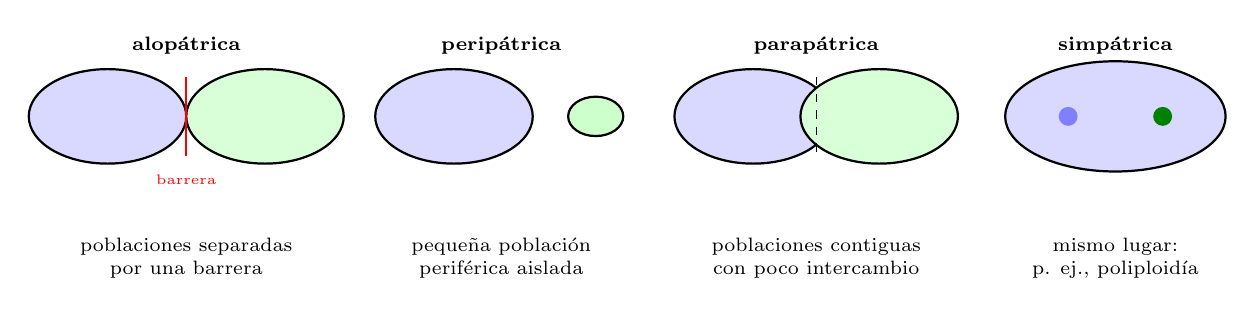
\begin{tikzpicture}
\tikzset{every node/.append style={align=center}}

\def\pop#1#2#3{\draw[thick, fill=#3] (#1,#2) ellipse (1.0 and 0.6);}
\node[font=\bfseries\scriptsize] at (1.4,4.3) {alopátrica}; \pop{0.4}{3.4}{blue!15}\pop{2.4}{3.4}{green!15}\draw[red, thick] (1.4,3.9) -- (1.4,2.9); \node[font=\tiny, red] at (1.4,2.6) {barrera};
\node[font=\bfseries\scriptsize] at (5.4,4.3) {peripátrica}; \pop{4.8}{3.4}{blue!15}\draw[thick, fill=green!20] (6.6,3.4) ellipse (0.35 and 0.25);
\node[font=\bfseries\scriptsize] at (9.4,4.3) {parapátrica}; \pop{8.6}{3.4}{blue!15}\pop{10.2}{3.4}{green!15}\draw[dashed] (9.4,3.9) -- (9.4,2.9);
\node[font=\bfseries\scriptsize] at (13.2,4.3) {simpátrica}; \draw[thick, fill=blue!15] (13.2,3.4) ellipse (1.4 and 0.7); \fill[blue!50] (12.6,3.4) circle (0.12); \fill[green!50!black] (13.8,3.4) circle (0.12);
\node[font=\scriptsize, align=center] at (1.4,1.6) {poblaciones separadas\\ por una barrera};
\node[font=\scriptsize, align=center] at (5.4,1.6) {pequeña población\\ periférica aislada};
\node[font=\scriptsize, align=center] at (9.4,1.6) {poblaciones contiguas\\ con poco intercambio};
\node[font=\scriptsize, align=center] at (13.2,1.6) {mismo lugar:\\ p. ej., poliploidía};

\end{tikzpicture}
\end{document}
